
\documentclass{article}
\usepackage{graphicx} % Required for inserting images
\usepackage{amsmath}
\usepackage{amsfonts}
\usepackage{amssymb}
\usepackage{bm}
\usepackage[top=1.3 in, bottom=1.2in]{geometry}
\usepackage{physics}
\usepackage{fancyhdr}
\usepackage{pgfplots}
\usepackage{siunitx}
\usepackage{braket}
\usepackage{mhchem}
\usepackage{chemfig}
\usepackage{gensymb}
\newcommand{\ve}{\mathbf}
\newcommand{\pa}{\partial}
\newcommand{\la}{\langle}
\newcommand{\ra}{\rangle}

\title{Ising Model Notes}
\author{Lachlan Kan}
\date{March 2025}

\begin{document}
\maketitle
\section{Introduction}
The Ising model describes the interaction between neighbouring spins on a lattice
under an external magnetic field. It is used to study the polarisation of ferromagnetic 
materials and how they align with an external magnetic field. Let us begin with 
a 1D chain of lattice sites from site 0 to site $N$. We know that each site can only interact with its nearest neighbours, and that 
the energy depends on how different their spins are. To model this, we say that 
\begin{align}
    \hat{H}_{int,\ n}\propto\hat{S}_z^n \hat{S}_z^{n+1}
\end{align}
Where the product is our measure of their difference in spins.
 In a lattice with $N$ sites, we can add this up to find 
the total interaction energy (Since it is indexed from 0, a lattice with $N$ sites 
will have indices from $0$ to $N-1$). 
Notice that when $n=N-2$, the interaction term will automatically include the $N-1$th site due to 
the $n+1$ present there. 
\begin{align}
    \hat{H}_{int}=-J\sum_{n=0}^{N-2}\hat{S}_z^n \hat{S}_z^{n+1}
\end{align}
Where the constant of proportionality is the coupling constant $J$. It is customary to append a negative sign due to convention. 
Suppose we subject the lattice to an external magnetic field of strength $h$, which tends to 
magnetise the lattice, influencing their spins along the $x$ direction. This energy can thus be 
found by 
\begin{align}
    \hat{H}_{ext}=-h\sum_{n=0}^N\hat{S}_x^n
\end{align}
Where the negative sign is once again due to convention. 
To find the total energy, we simply sum the energies from (2) and (3), giving 
\begin{align}
    \hat{H}=-J\sum_{n=0}^{N-2}\hat{S}_z^n \hat{S}_z^{n+1}-h\sum_{n=0}^N\hat{S}_x^n
\end{align}
Notice that the hamiltonian consists of two competing terms trying to influence the spins of the electrons: the interaction term and the field term. 
When $J>>h$, the interaction term takes over, 
and the spin will be aligned along the $z$-axis. Conversely, when 
$h>>J$, the field will be strong enough to overpower the interactions, 
leaving the spins aligned 
along the field in the $x$-axis. 

\section{Spins Operators of electrons}
Now, to use this hamiltonian, we first have to find each $S_z^n$ associated with the $n$th site. 
To do this, we make use of the Pauli $z$ matrix, $S_z$. For example, for 3 lattice sites, we say that 
\begin{align*}
    \hat{S}_z^0&=\hat{S}_z\otimes I\otimes I\\
    \hat{S}_z^1&=I\otimes \hat{S}_z\otimes I\\
    \hat{S}_z^2&=I\otimes I\otimes \hat{S}_z
\end{align*}
For the case of 3 lattice sites, we have 3 tensor products to obtain each spin. Notice that the spin is only described by the Pauli matrix when its at its own index
(The one for spin 0 has $\hat{S}_z$ at the 0th place, the one for spin 1 has $\hat{S}_z$ at the 1st place, etc.). This is equivalent 
to saying "there is only a component of spin at the site where the index matches 
the location of the particle". Therefore, the spin operator acts non-trivially only on its corresponding site, and as identity elsewhere.
This can be generalised to higher numbers of sites, but generally, for $N$ sites, 
there will be $N$ tensor products per site to compute the spins. To compute the $x$ spin in 
the second term, we repeat the above process,
 replacing the Pauli $z$ matrix with the Pauli $x$ matrix. 
\section{Energy Levels}
To find the energy levels, we need to solve the Schrodinger equation for its energy eigenvalues $E$, which is as follows 
\begin{align}
    \hat{H}\ket{\psi}=E\ket{\psi}
\end{align}
This is an eigenvector-eigenvalue equation, where $\ket{\psi}$ represents the state of the whole lattice, and $\hat{H}$ is given in (4).
Computing the hamiltonian for $N$ lattice sites should give an $2^N\cross 2^N$ matrix. This means computing the various 
energy eigenvalues $E$ will be an exponentially more arduous task with every increasing $N$. Solving for the eigenvalues $E$ will give the 
energy levels, while solving for the eigenvectors $\ket{\psi}$ gives the state of the whole lattice.

\section{Computing the Spins}
The spins of each site can either be up or down. For simplicity and 
ease of computation, we will assign electrons 
a spin of $\pm1$ (See appendix). Spin up will be 
assigned to $+1$ and spin down to $-1$. To obtain this spin, we first find the expectation value of the $\ket{\psi}$ computed in the last section 
when applied to by $\hat{S}^n_z$ (computed in section 2), which gives 
\begin{align}
    S^n_z=\bra{\psi}\hat{S}^n_z\ket{\psi}
\end{align}
This gives the $z$ spin for the $n$th electron. 
Applying this formula to each electron from $n=0$ to $n=N$ will give the spins to all the electrons. To find the $x$-spin, 
the same process can be repeated but with the $\hat{S}^n_x$ computed in section 2.

\section{Ising Model in 2 Dimensions}
The Ising model can be further generalised into 2 dimensions. Now, for any 
given site $i$, 
the electron can interact with any of its nearest neighbour 
sites $j$. The Hamiltonian, under no external magnetic field, now reads 
\begin{align}
    \hat{H}=-J\sum_{\la i,j\ra}\hat{S}_z^i \hat{S}_z^{j}
\end{align}
Each site is specified by a set of coordinates ($x,y$) 
since the lattice is now a 2D grid of sites (Note that in the Python code, $x$ and $y$ are replaced by $i$ and $j$ because 
I've gotten used to using $i$ and $j$ for 
indices inside loops and I don't intend to change that. 
The index number in the code is specified by $n$ and the coordinates by $i$ and $j$.
 There is no $x$ and $y$ anywhere in the code. Don't go looking for it). 

\section{The Monte-Carlo Method}
Obviously, solving (7) via direct diagonalisation is impossible. The 1D strip has a
Hamiltonian matrix of 
size $2^N\cross 2^N$, and in 2D, we need to compute not just $N$, but $N^2$ sites. Hence the 
Hamiltonian matrix of (7) will have dimensions $2^{N^2}\cross 2^{N^2}$ - a ridiculously large number that 
 even the best supercomputers of the world will run into problems trying to solve for a relatively small lattice. 
With this, its safe to say that we need a new method of calculating the stable
 energies and spins of the system.
  Evidently we can't directly treat all the electrons, but what we can do, is look for a 
  classical approximation for their interactions. 
We randomly sample $some$ electrons and calculate the energy for their interactions. 
It is easy to see that for a large enough sample size, 
the interactions of this sampled group will be somewhat 
representative of the exact solution. This is where Monte-Carlo comes in. 
\subsection{Side Quest - Approximating $\pi$}
To get a feel for the Monte-Carlo method, lets consider a totally separate problem - approximating $\pi$. 
If we draw a square with side lengths $r$, and then inscribe a quarter circle inside that square, we know that 
the ratio of areas between the square and quarter circle will be as follows. 
\begin{align}
    R=\frac{A_{O}}{A_{\square}}=\frac{\frac{1}{4}\pi r^2}{r^2}=\frac{1}{4}\pi\implies \pi=4R
\end{align}
Where $A_O$ denotes the area of the quarter circle, not a full circle. Now if we have the areas 
of the quarter circle and the square, then the exact value of $\pi$ can be easily found. However, we don't. 
So how can we find these areas? One way to approximate the area is to draw the square circle combination on a piece 
of paper and sprinkle sand evenly onto the paper. When the sand covers roughly the whole sheet, 
we can then count the grains of sand inside the quarter circle, then count the 
total grains of sand inside the square, and then divide the two to find the ratio. The reason for doing this 
is because the number of sand grains the quarter circle can hold is directly proportional to the area of the
 quarter circle, and the grains of the square is proportional to its area as well, so dividing the two numbers is a good representative of the ratio of their areas. 
Of course, counting grains of sand is unrealistic 
(probably a task for a professor's team of graduate students), 
and so we leave this mundane task to the computer. 
$\\\\$
\noindent To implement this on a computer, 
we can generate a random set of points $P_i(x_i,y_i)$, which 
represents the random positions of all the grains of sands. Then, we can compute each points' radial distances from the origin (which we set to be one corner of the paper, at the center of the quarter circle), 
$d_i=\sqrt{x_i^2+y_i^2}$. It is easy to see that for the $i$th point, if it lies inside the circle, then $d_i\leq r$. Conversely, if $d_i>r$, 
then the point lies outside of the circle. We can thus approximate $\pi$ by quadrupling the ratio of the number of 
points of which $d_i\leq r$ to the total number of points. 
We can see how accurate this approximation is by implementing this algorithm, and then plotting 
the value of the approximation to the number of "grains of sands dropped" (iterations). Doing so, 
we obtain figure 1.
\begin{center}
    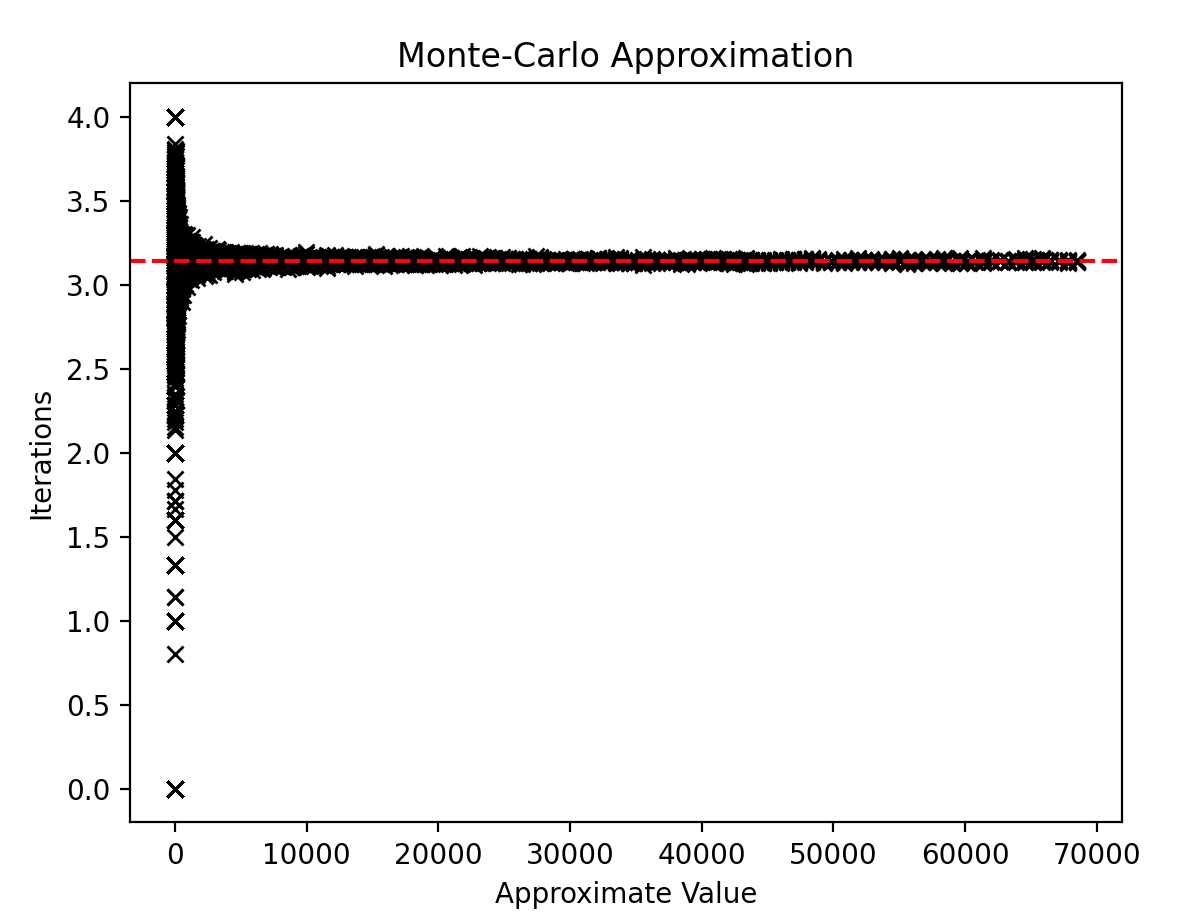
\includegraphics[scale=0.43]{monteCarlo.png}\\
    (Fig. 1)
\end{center}
Our best approximation was $\pi=3.1415753$, which is not that far off (an error of $1.73\cross10^{-5}$)! On the graph, 
the actual value for $\pi$ is denoted by the red line. 
We see that the approximation is horrible for small iterations, 
but get much better for large numbers. 
This is because of the fact that the error goes like $\delta\sim1/\sqrt{N}$, so 
for the Monte-Carlo approximation to be any good, we must run many many iterations. 
\subsection{The Metropolis Algorithm}
To apply this method to our problem, we can randomly sample each lattice site and calculate their interactions. However, 
we immediately run into a problem - to calculate the interactions of any particular lattice site,
we must know the spins of its neighbours! And to obtain the spins of the neighbours, we must calculate their interactions 
with the neighbours neighbours! And this goes on and on until we have to exactly calculate for the whole lattice - which we cannot do. 
So how to we calculate the interaction of a single site 
without knowing the details of its neighbours? 
Again, we turn to another classical approximation. This is where the Metropolis Algorithm comes in. 
$\\\\$
\noindent Suppose we have a lattice with sites that has totally random spins. 
Since we know the spins (they are random), the Hamiltonian of (7) reduces to a simple numerical 
value for the energy 
(there is no need to diagonalise the Hamiltonian to obtain the spins, 
we know them already). If there is no external magnetic field, the total 
energy can thus be found by
\begin{align}
    E=-J\sum_{\la i,j\ra}S_iS_j
\end{align} Now, we can randomly sample each lattice site, and try to flip the spin.
 After we flip the spin,
we calculate the energy again. 
Intuitively, we know that 
any natural system is likely to move to a lower energy state. Therefore, 
if the new energy is less than or equal to the old 
energy, then we confirm that the spin is flipped, and move on to try and flip the next (random) one. If the new energy 
is greater than the old one, then the spin is not likely to flip. To do this, we can compute 
the old energy and new energy in every iteration to find the change in energy. 
However, that is not very efficient since the energy has to be recomputed twice every 
iteration, meaning the computer has to add up the spins from all $N\cross N$ lattice site twice. 
So lets find an expression for $\Delta E$ that dosen't require this computation. 
$\\\\$
\noindent We can represent the electron $S_i=S_{x,y}$ at site $i=(x,y$) flipping by $S_{i}\to-S_{i}$. We know that this will 
affect only the terms that have $S_i$ as a factor, namely the terms containing its nearest neighbours. We can write out the affected terms as follows 
\begin{align}
    f=S_{x,y}S_{x+1, y}+S_{x-1, y}S_{x,y}+S_{x,y}S_{x, y+1}+S_{x,y-1}S_{x,y}
\end{align}
Following the spin, $f$ will also flip signs because all the $S_i$ inside has 
its sign flipped. We can subtract the terms $Jf$ from the energy,
 which gives the part of the energy that 
remains unaffected by the electron flip. 
Following this, we can add $-Jf$, which is the new 
part of the energy to the system. Overall, we obtain an expression 
for the new energy, which we denote by $E'$ as follows
\begin{align}
    E'=-J\sum_{\la i,j\ra}S_iS_j-Jf+(-Jf)=E-2Jf
\end{align}
The change in energy can then be found as 
\begin{align}
    \Delta E=E-E'=2Jf=2JS_{s,y}(S_{x+1,y}+S_{x-1,y}+S_{x,y+1}+S_{x,y-1})
\end{align}
We can then use the sign of this change in energy to determine whether or
 not a flip is allowed to occur. Again, a flip that causes $\Delta E \leq0$ is likely to happen, while 
 a flip that causes $\Delta E>0$ is not.  
However, a flip that raises the energy is not impossible. 
Due to the probabalistic nature of statistical mechanics, the
 probability of an energy raising
 flipping can be described by the Metropolis probability, $P=\exp(-\Delta E/k_BT)$. 
 Notice that the flips that raise energy becomes exponentially less 
 likely for higher and higher changes in energies. 
Notice also, that it is dependent on the temperature $T$. 
For low temperatures, the algorithm is less likely to accept flips while 
for high temperatures, a flip is more easily accepted.
\noindent In summary, 
for every flip, 
\begin{align}
    \begin{cases}
    \Delta E\leq0&\implies \text{Flip accepted}\\ 
    \Delta E>0&\implies P=\exp(-\frac{\Delta E}{k_BT})\text{ To accept flip}
    \end{cases}
\end{align}
We can repeat this algorithm many times for random lattice sites until a stable 
state is reached (a state 
where no further flips are accepted).
For very low temperatures ($T\to0$),  The energy of this state will approach 
the ground state energy eigenvalue, and this state is 
the ground state spin configuration that we are looking for. 
$\\\\$
\noindent This algorithm is much faster than doing direct diagonalisation by many orders of magnitudes. However, 
for larger and larger lattices, convergence will be increasingly slow, and the number of iterations taken will be higher and higher. 
For perspective, the convergence of a 25$\cross$25 lattice took my computer 39640 iterations! In practice, the calculations 
of actual lattices (which may be millions of sites wide!
 Since each site represents one single electron)
  is done on world class supercomputers for months on end!
$\\\\$
\noindent Implementing this algoritm ($J=1,\ T=10^{-18}$), we first start with the random lattice on the left, 
and as iterations go by, we arrive at the partially magnetised one in the middle, and eventually the 
fully magnetised one on the right (Blue represents spin up while red represents spin down). 
\begin{center}
    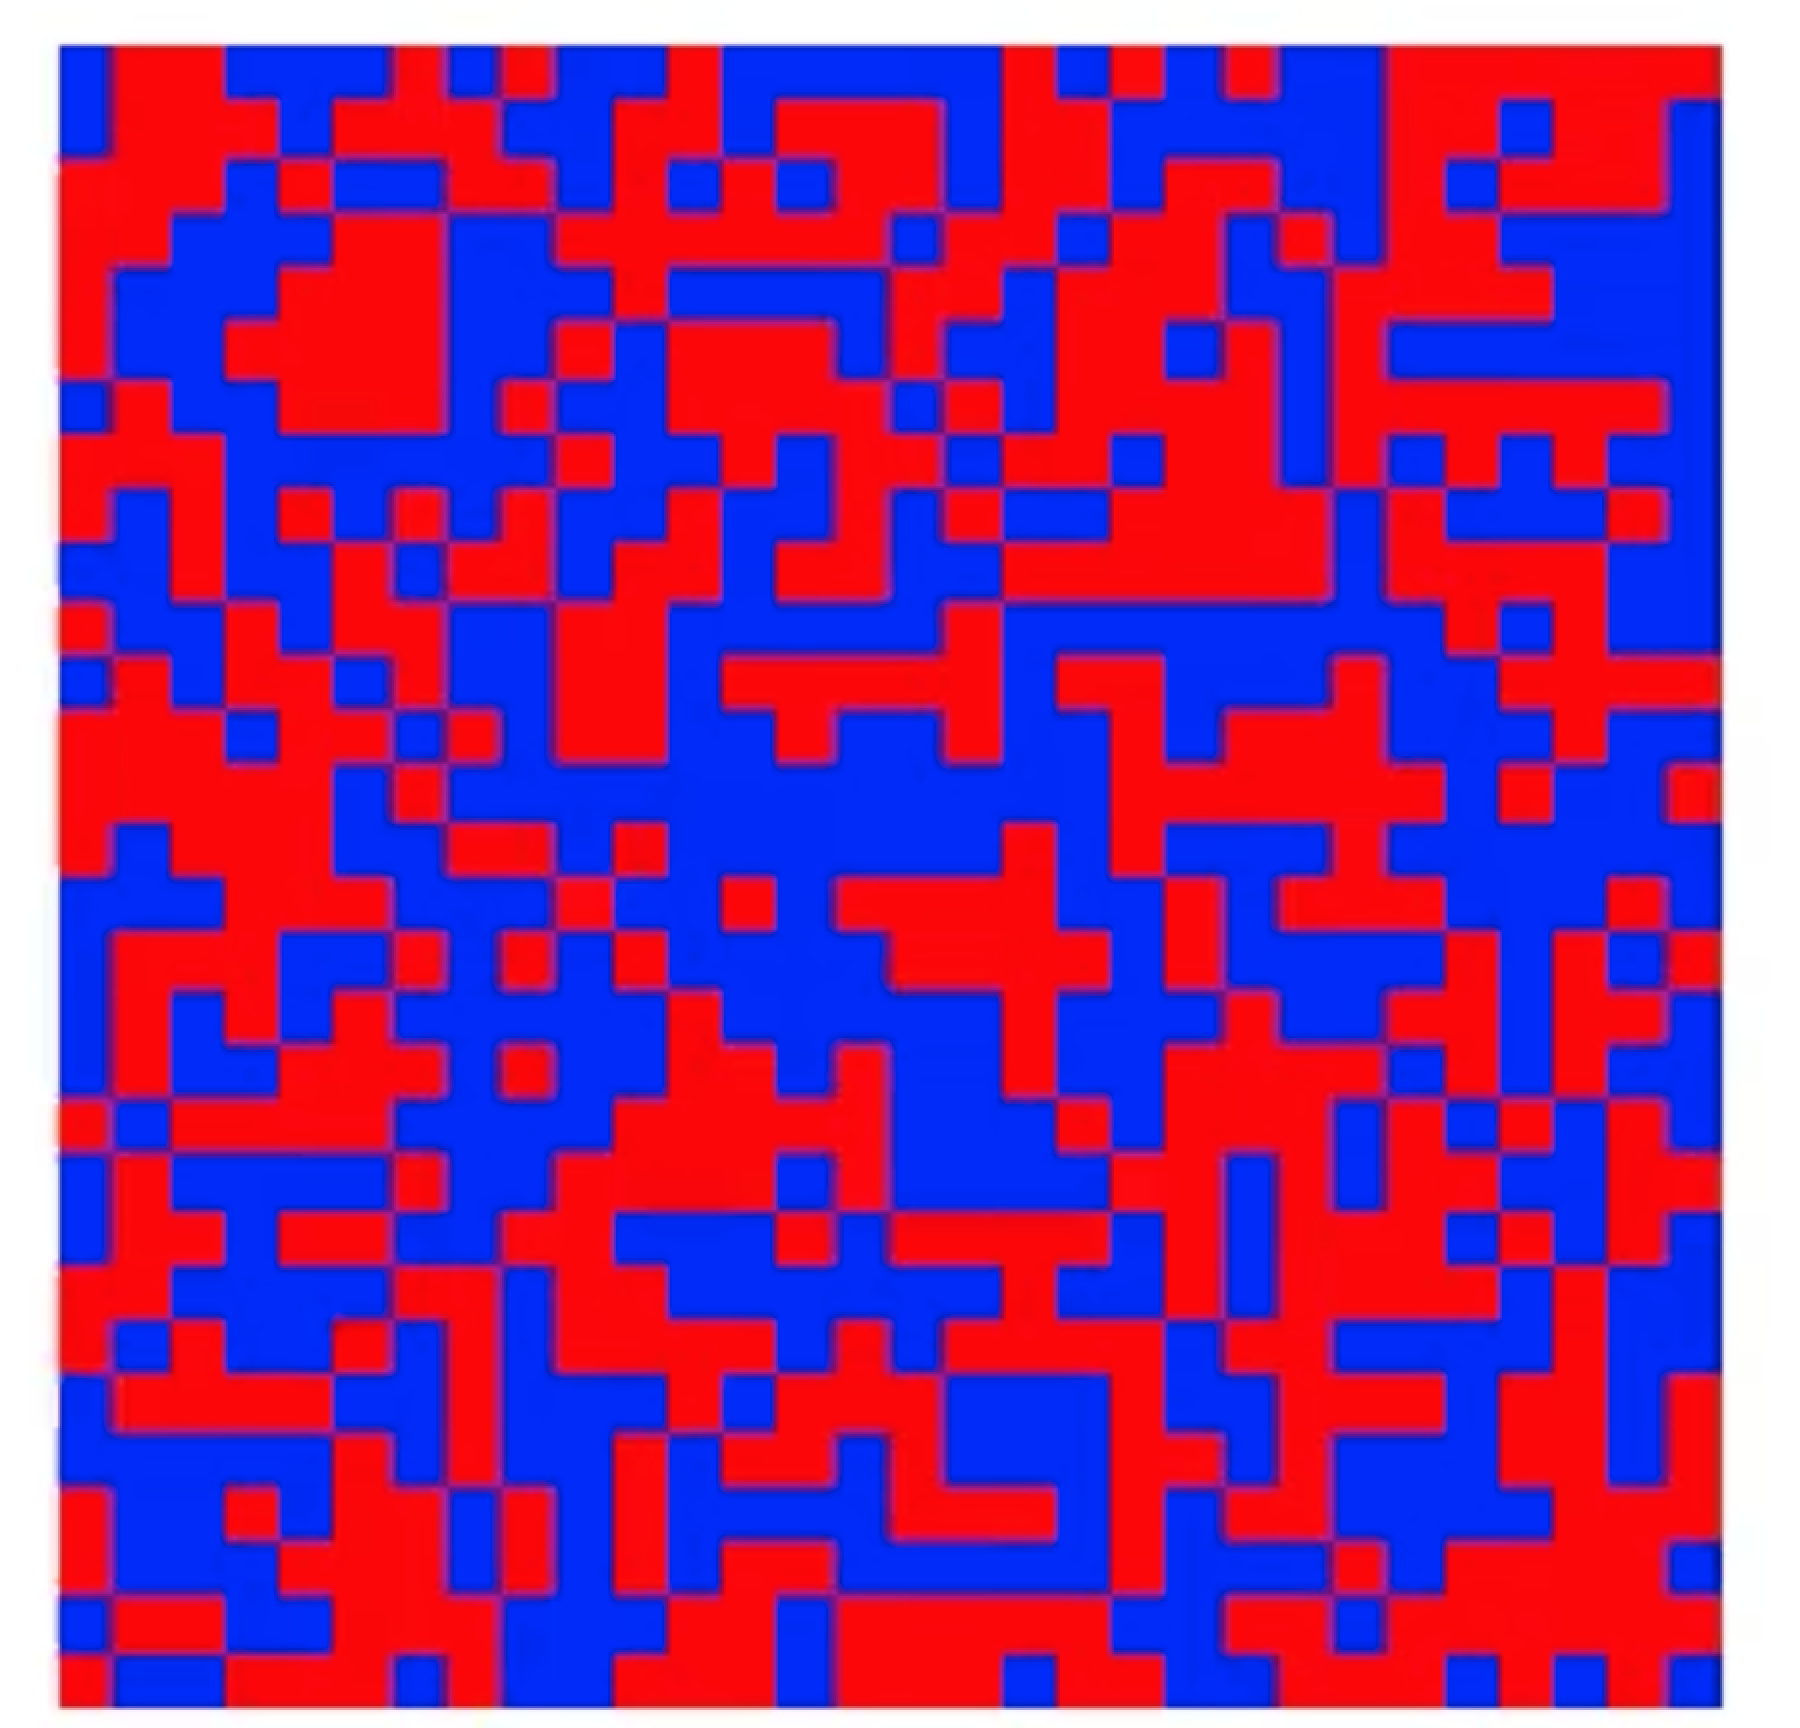
\includegraphics[scale=.1]{noAlign.png}\ 
    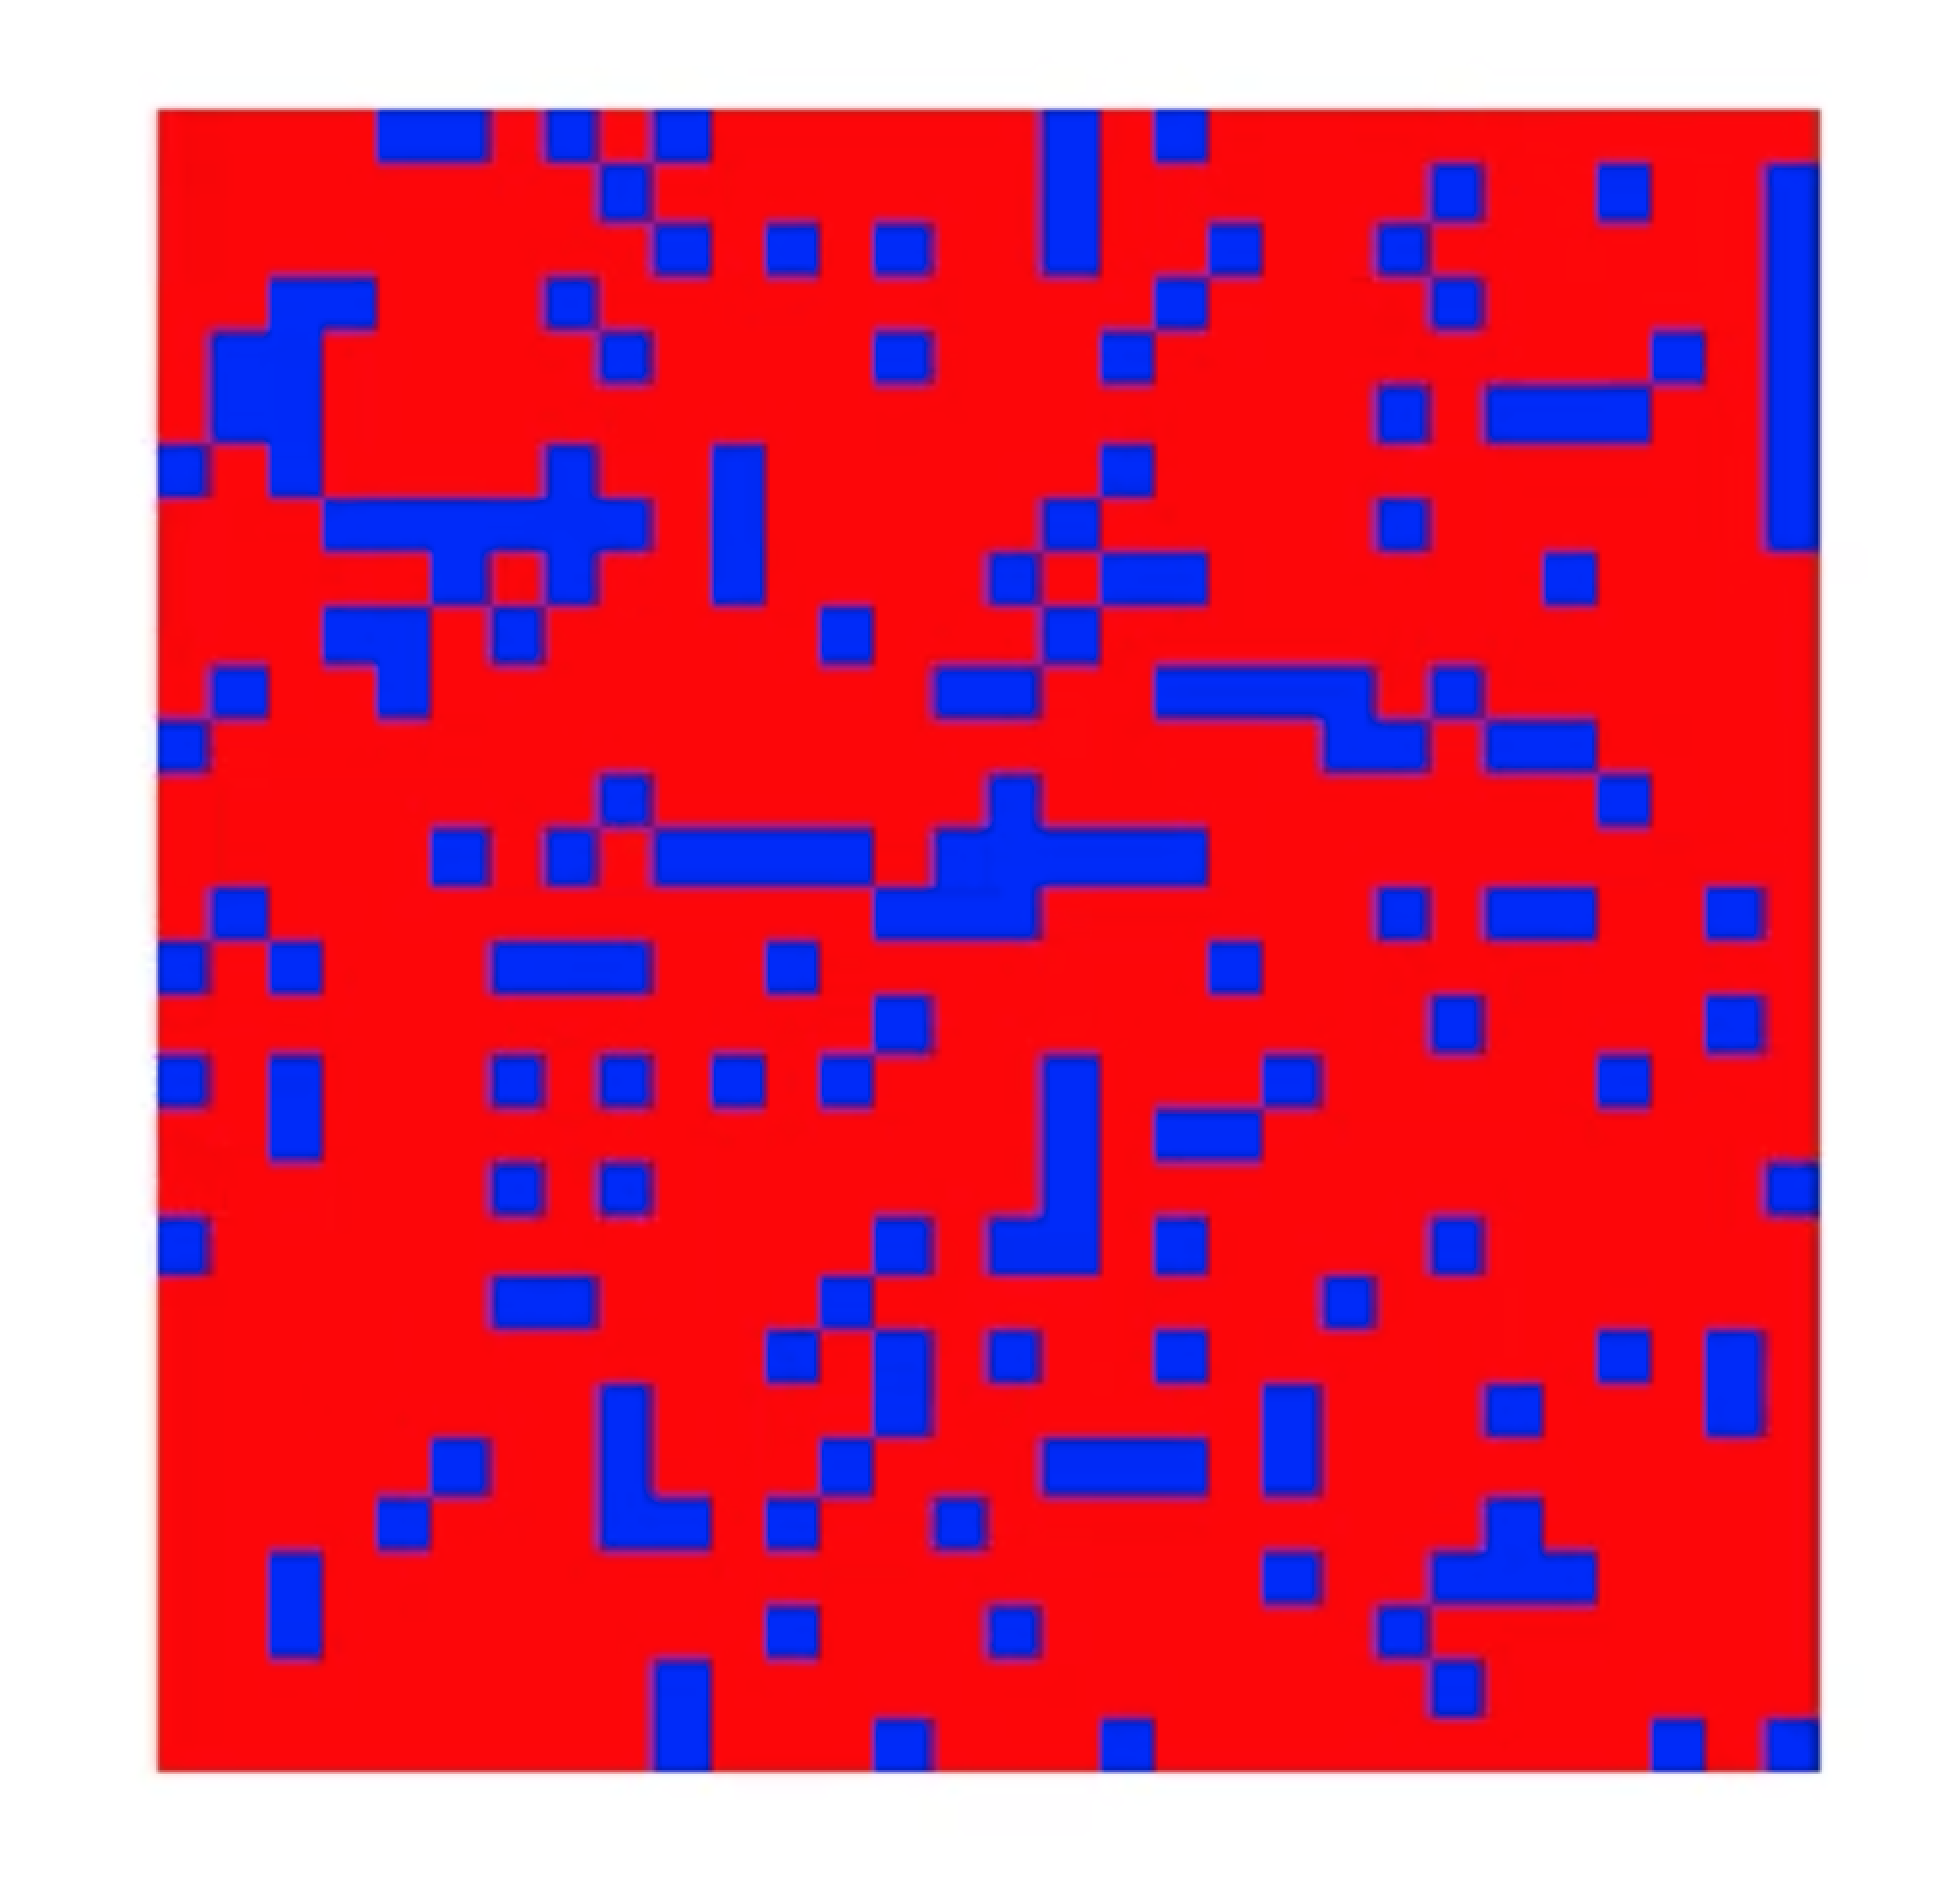
\includegraphics[scale=.1]{partAlign.png}\ 
    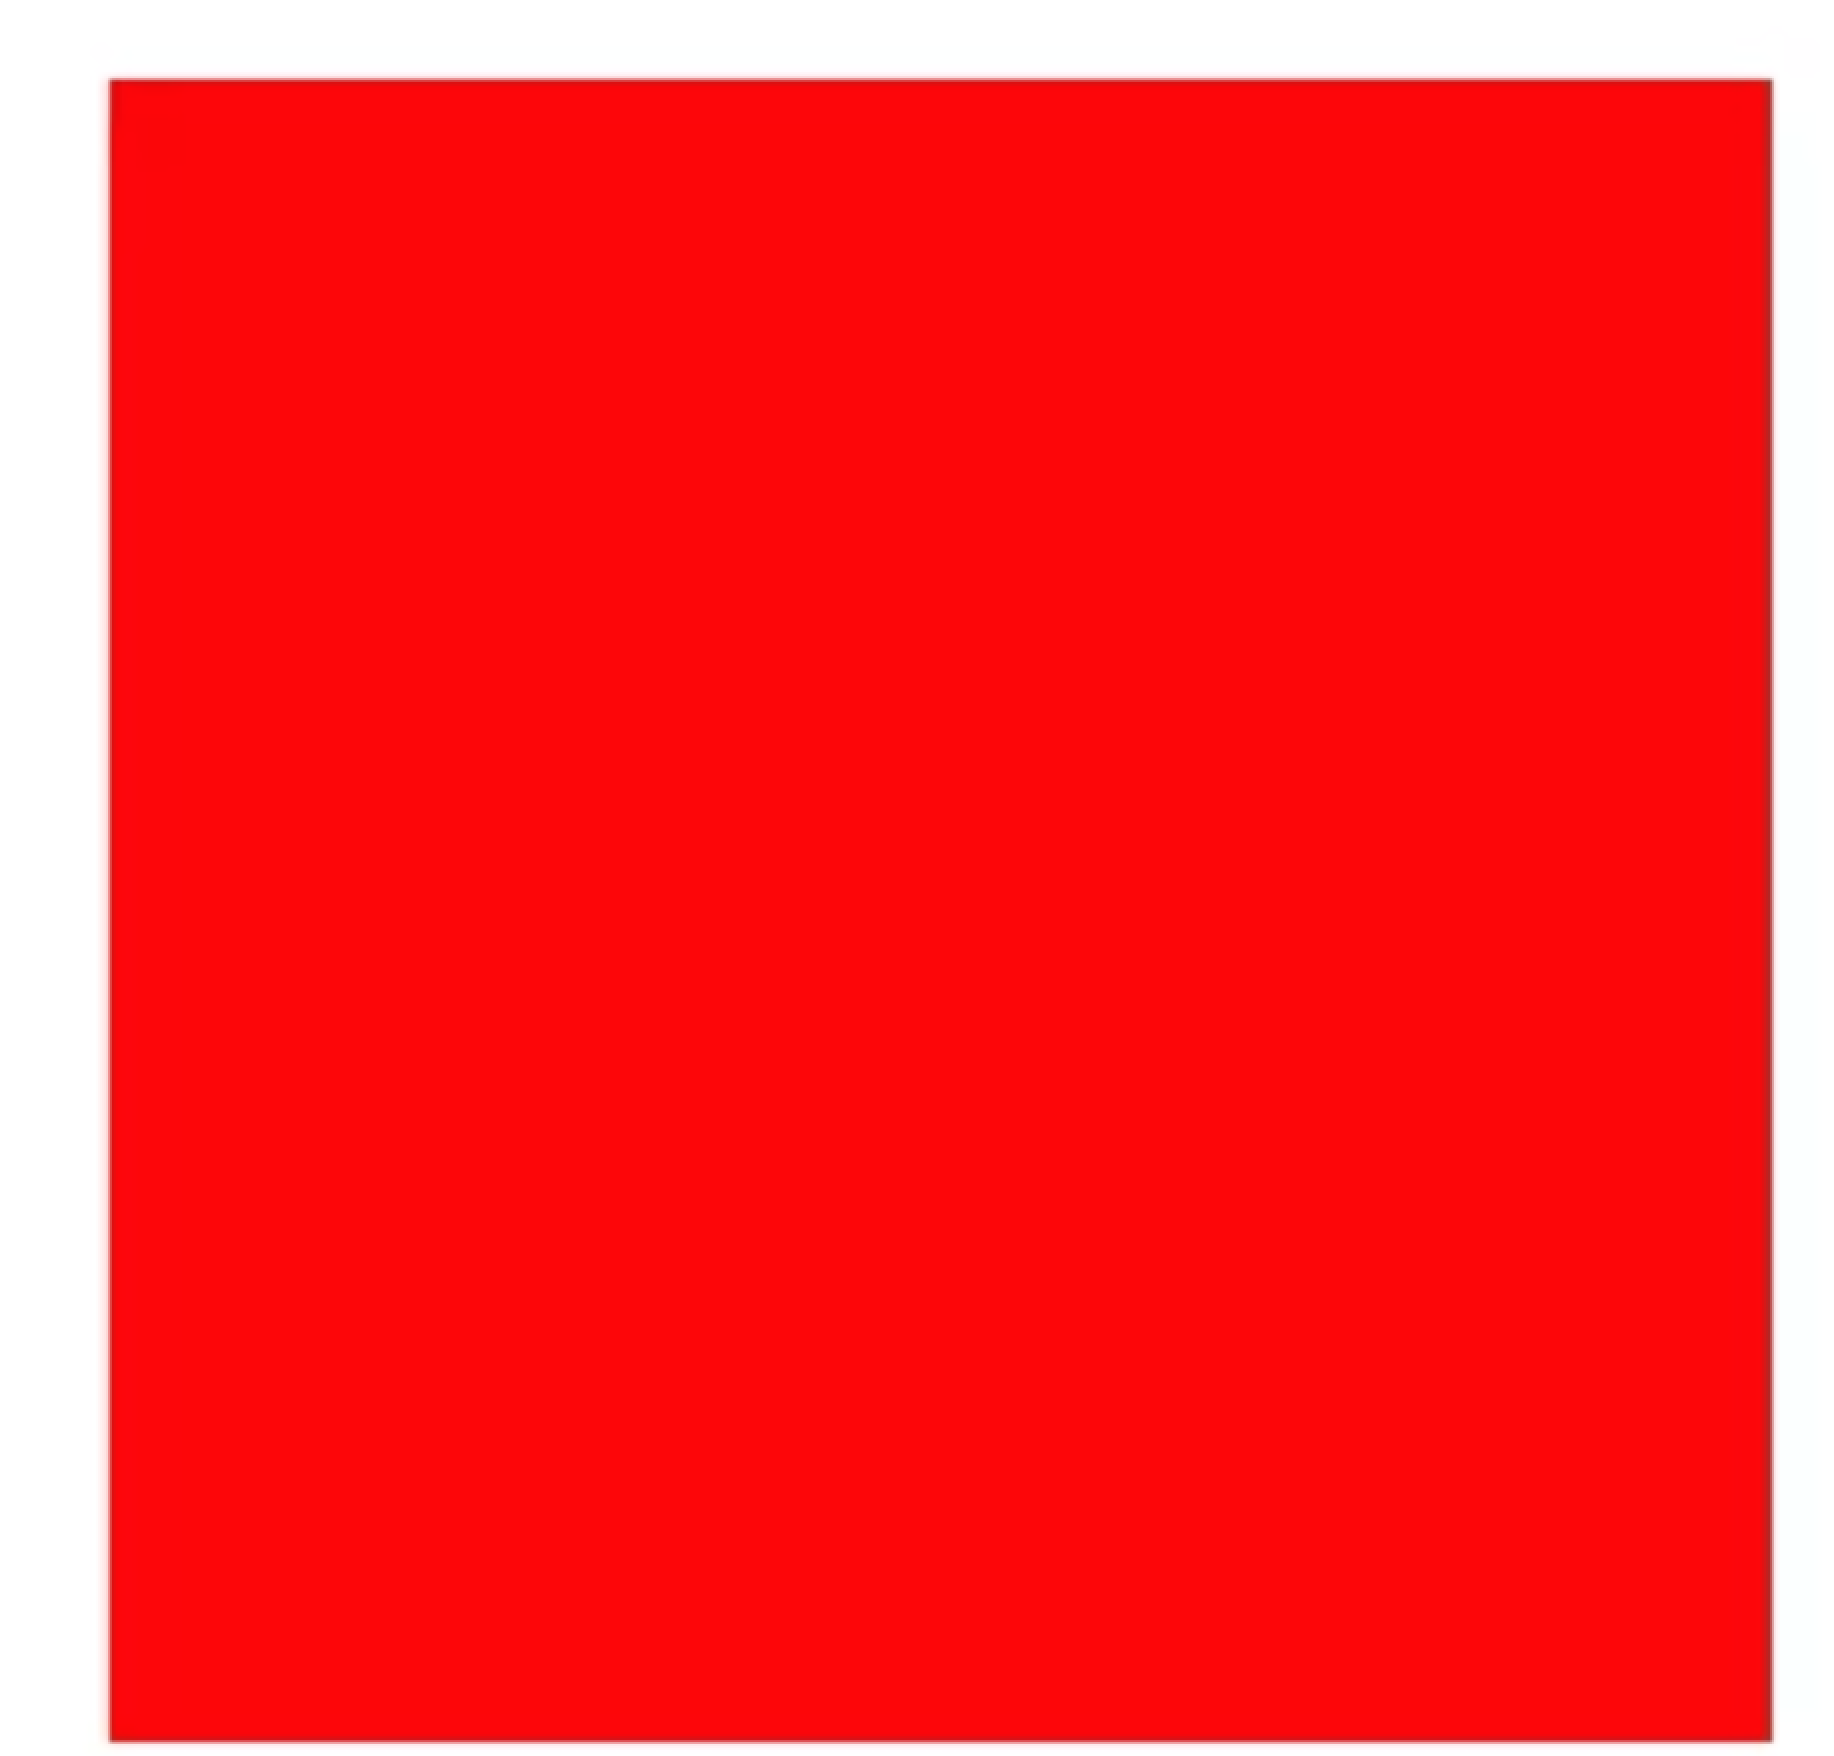
\includegraphics[scale=.1]{fullAlign.png}\\[-3.9pt] 
    (Fig. 2)
\end{center}
Since the speed of convergence scales with lattice size, this (30$\cross$ 30)
is the largest lattice that my computer can bring to full convergence in a 
reasonable amount of time. We see that convergence happens when all spins are the same (aligned).
We can thus try to work out this minimum energy. Since $i$ and $j$ are nearest neighbour sites with two coordinates $(x,y)$, 
we can expand our sum in (9) to 
\begin{align}
    E=-J\sum^N_x\sum^N_yS_{x,y}(S_{x+1,y}+S_{x,y+1})
\end{align}
Here, we sum to $N$ and implement periodic boundary conditions, where the $N+1$th site 
loops back to the 0th site. Notice that regardless of the sign of the spins, the product is always positive if 
they are to be all the same. Hence, (14) becomes 
\begin{align}
    E=-J\sum_x^N\sum_y^N\pm1(\pm1\pm1)=-J\sum_x^N\sum_y^N2=-2JN^2
\end{align}
Under temperatures of near 0, this should be the energy that 
the system converges to. Now, for our run, we can also how the energy changes over the coruse of the
whole process, as shown in figure 3.
\begin{center}
    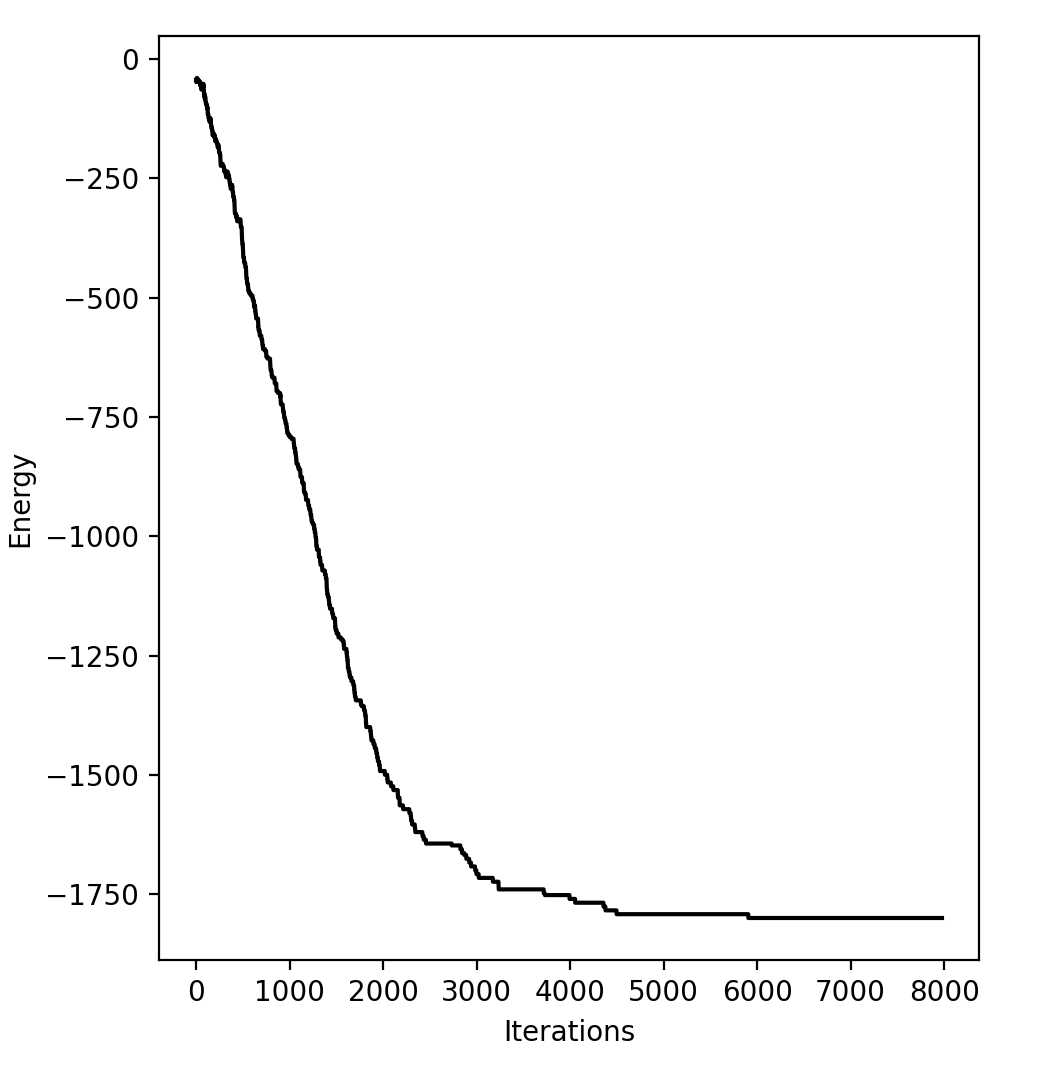
\includegraphics[scale=.45]{energy_noMag.png}\\ 
    (Fig. 3)
\end{center}
Indeed, it converges to $-2\cross1\cross30^2=-1800$, which is expected. Notice how jagged this curve is, and in some parts, the energy even goes up! However, 
since I set the temeprature very low to make convergence possible (in a reasonable amount of time)
, the "going up" 
effects aren't all that visible unless you zoom in really hard. If we want 
the stochastic part to be more visible, we can increase the temperature to let more energy raising flips through. 

\section{Temperature and Magnetisation}
Here is where the interesting property of magnetism comes in. It is well known that 
when more spins are aligned, the object will behave magnetically. We can measure this 
ability to interact with the magnetic field by a quantity known as magnetisation. Here, 
each spin can either be $+1$ or $-1$, so if two qubits have the same spin, 
we can add them up
to either $\pm2$ depedning on their sign,
 which means the overall effect is a stronger magnetisation, 
since the magnitude is increased. Conversely, if they have different signs, then it will add 
up to 0, since the spins cancel each other out.
 We can generalise this idea to add up all the spins 
of the electrons in the lattice to obtain the total magnetisation $M$ as follows 
\begin{align}
    M=\sum_{i}S_i
\end{align}
Which is the proper definition for magnetisation. We can now figure out how magnetised our 
lattice is by first determining the equilibrium lattice as found above, and then 
calculating the magnetisation the same way of how we found (15). If our temperature is sufficiently low, then 
there will be negligible thermal fluctuations.  This means that the equilibrium state will 
be comprised of a lattice filled with electrons of the same spin. Hence we can easily 
work out the sum in (16) if we sum to $N$ and implement the same periodic boundary conditions. 
\begin{align}
    M=\sum_i(\pm1)=\pm N^2
\end{align}
The $N^2$ is due to the fact that we are summing over all sites $i$, and we have $N^2$ sites in our 2D square lattice.
This shows that as $T\to0$, we will be able to achieve maximum magnetisation $M\to\pm N^2$. Recall from last section that 
as temperature increases, the spins tend to not line up. Therefore, from a qualitative view, 
magnetisation should decrease as temperature increases, and that is exactly what happens...sort of. 
$\\\\$
We can test the relationship between temeprature and magnetisation by
simulating many lattices (using the methods introduced in previous sections) 
under a range of $T$, and calculate their magnetisations at the end. After all the calculations, 
we can plot $M$ and $T$ in the $y$ and $x$ axis respectively. Doing so, we obtain the
 following.  
\begin{center}
    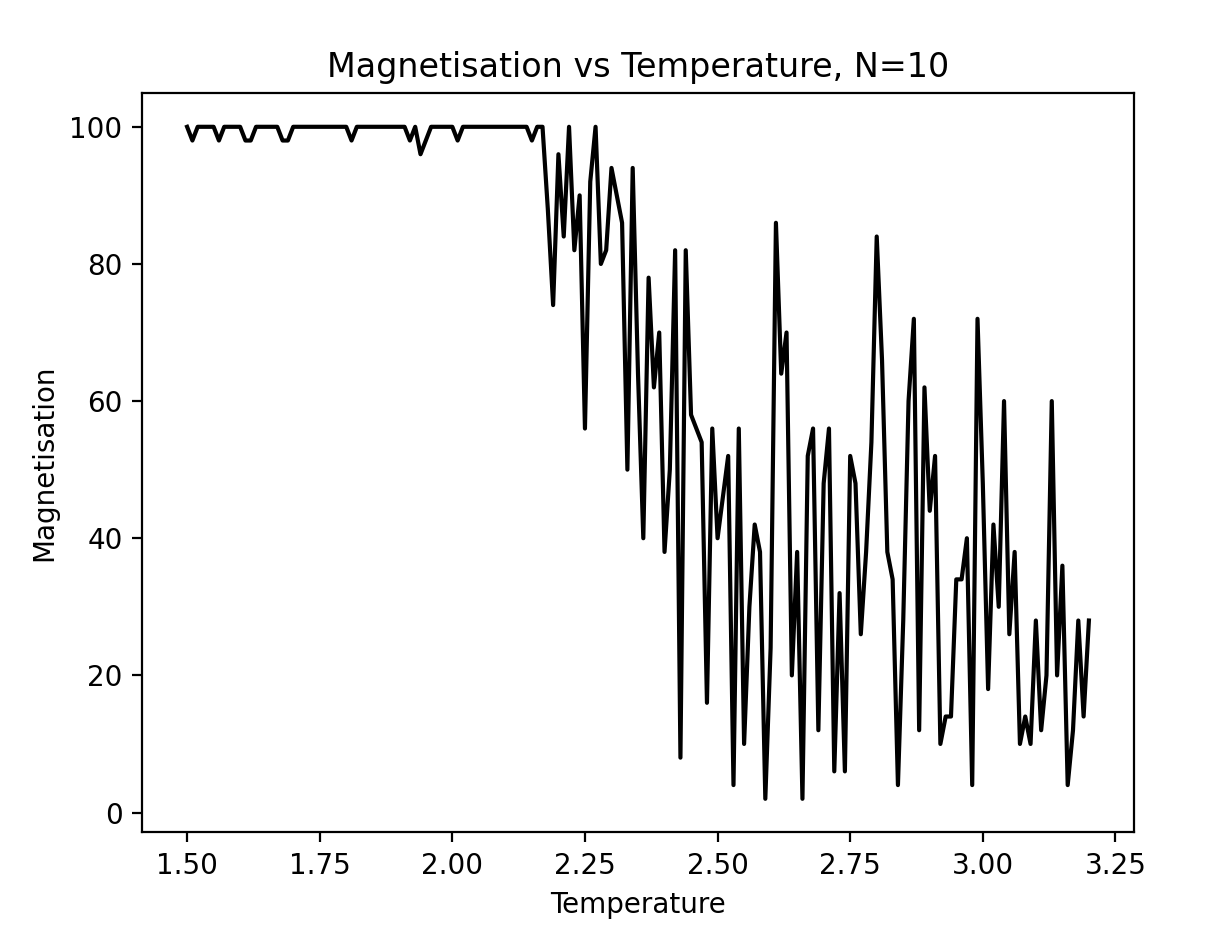
\includegraphics[scale=.5]{MagTemp_N=10.png}\\ 
    (Fig. 4)
\end{center}
Notice that when temperature is increased from near 0, the magnetisation dosen't seem to be too affected. However, 
past a certain point, magnetisation drops rapidly to near 0. This temperature is the "Curie Point", and 
is where ferromagnetic materials like iron typically lose their magnetism. In Osanger's 
exact solution, this point was determined to be at 2.269, which is close to our approximate
point, which is at about 2.20 (Which is impressive considering our lattice size is only 10).  It is also important to note that 
for large system $N\to\infty$, this drop happens as a discontinuity instead of just a rather steep slope as seen here. This is known as a "phase transition" as the 
lattice stops being magnetised. 



\section{External Magnetic Fields}
We can now start to include external magnetisation in our model. If we add the magnitisation 
term back into our total energy expression, we obtain 
\begin{align}
    E=-J\sum_{\la i,j\ra}S_iS_j-h\sum_iS_i
\end{align}
Where $h$ is the magnetic field strength we had at the start. Repeating our process which we used to find (10) for this energy, 
we can see that 
\begin{align}
    \Delta E=2S_i(Jf+h)
\end{align}
Here, we see that the magnetic field contributes to the energy difference. This means 
if $|h|$ is large, a very large number will be added to $\Delta E$. 
This causes $\Delta E$ to become large, forcing the probability of an energy increasing spin to be small. It can 
be thought of as a large magnetic field "forcing" the lattice to return to the ground state, 
since anything else is made exponentially unlikely by the $h$ term. Conversely, for small $|h|$, it can be seen that 
it has the opposite effect, promoting chaos and reducing convergence speed. We can see
this in action in our simulation. If we let $h=0.01$ (shown on th left) 
and compare its
results to $h=10^3$ (shown on the right), we obtain 
\begin{center}
    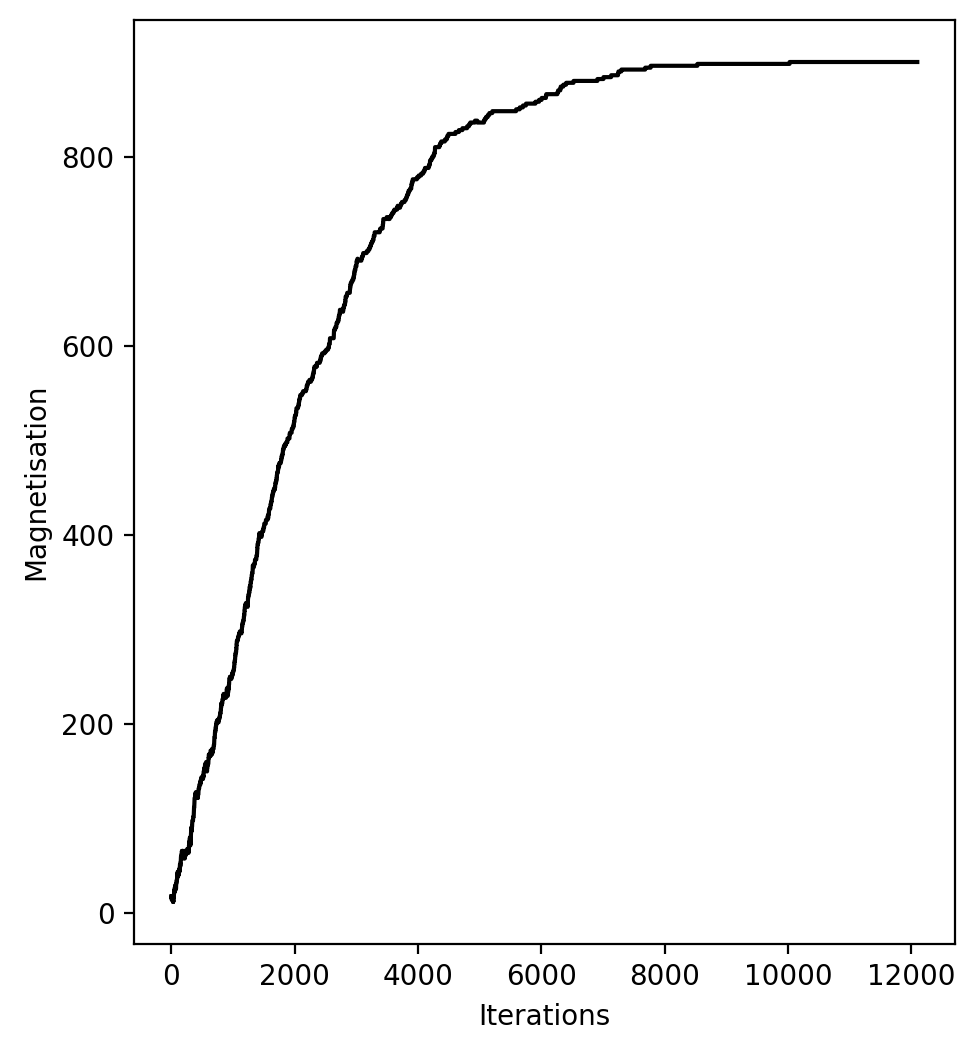
\includegraphics[scale=.33]{lowMag.png}\ 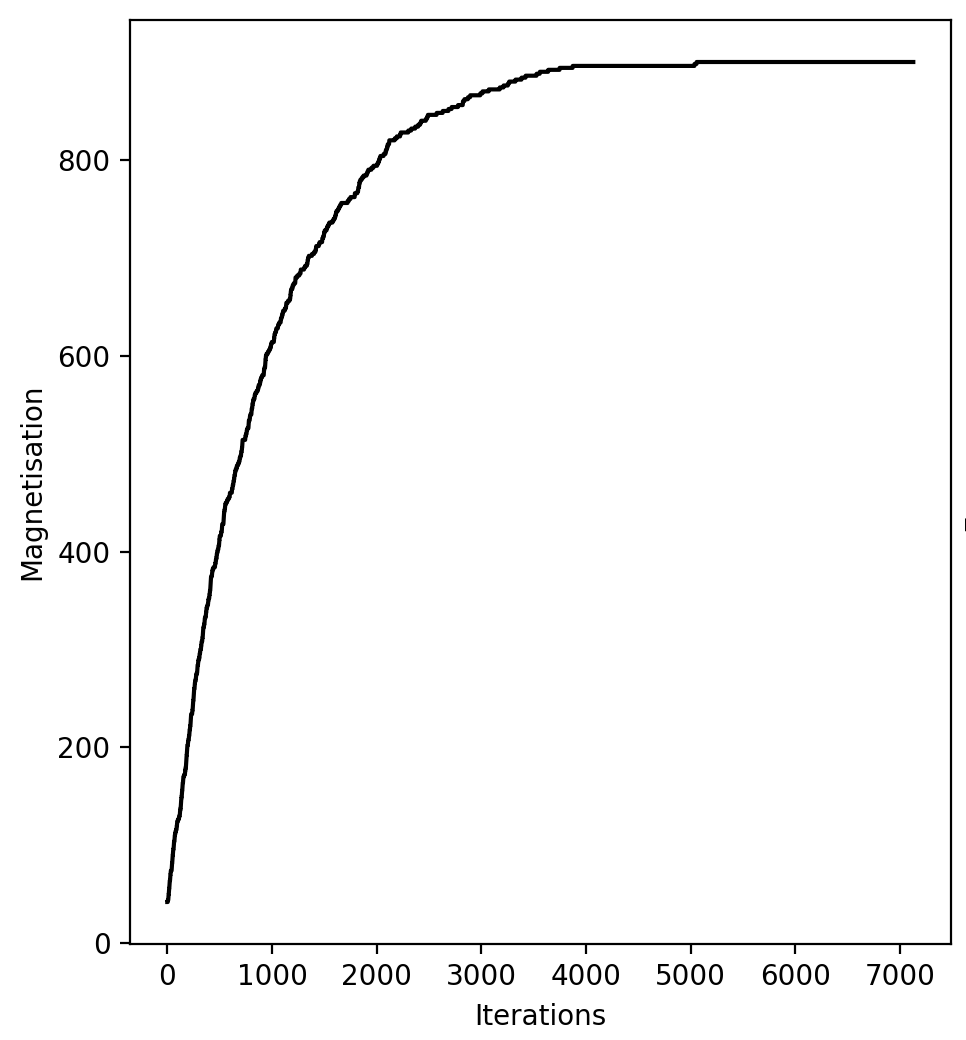
\includegraphics[scale=.33]{highMag.png}\\ 
    (Fig. 5)
\end{center}
Indeed, the one on the left has a much higher iteration count (at around 12000) compared to the one on the right 
(at around 7000), indicating a slow convergence. Another interesting point
 to note is that the left is more jagged (chaotic)
than the right, since the "forcing effect" from $h$ is much less. It is also not a surprise that for a large enough lattice where convergence is not always easy, that
a large magnetic field leads to high magnetisation, converging $|M| \sim  N^2$, while a weak magnetic 
field leads to smaller magnetisations $|M|<<N^2$ as the lattice becomes disuniform.
\section{Appendix: Pauli Matrices}
The Pauli matrices used in this set of notes are as follows. 
We will work in units where $\hbar=k_B=1$. 
\begin{align*}
    \hat{S}_x&=\begin{bmatrix}
        0 & 1\\ 
        1& 0
    \end{bmatrix}\\
    \hat{S}_y &= 
    \begin{bmatrix}
        0 & -i \\
        i & 0
    \end{bmatrix}\\ 
    \hat{S}_z&=\begin{bmatrix}
        1 & 0\\ 
        0 & -1
    \end{bmatrix}
\end{align*}
Although electrons (and all fermions) have half-integer spins,
I have opted for the electron spin here to be simplified to $\pm1$ to avoid floating point error in the Python program. 

\end{document}